\documentclass[crop,tikz]{standalone}
\tikzstyle{bag} = [align=center]
\usetikzlibrary{positioning}
\usetikzlibrary{arrows.meta}

\begin{document}
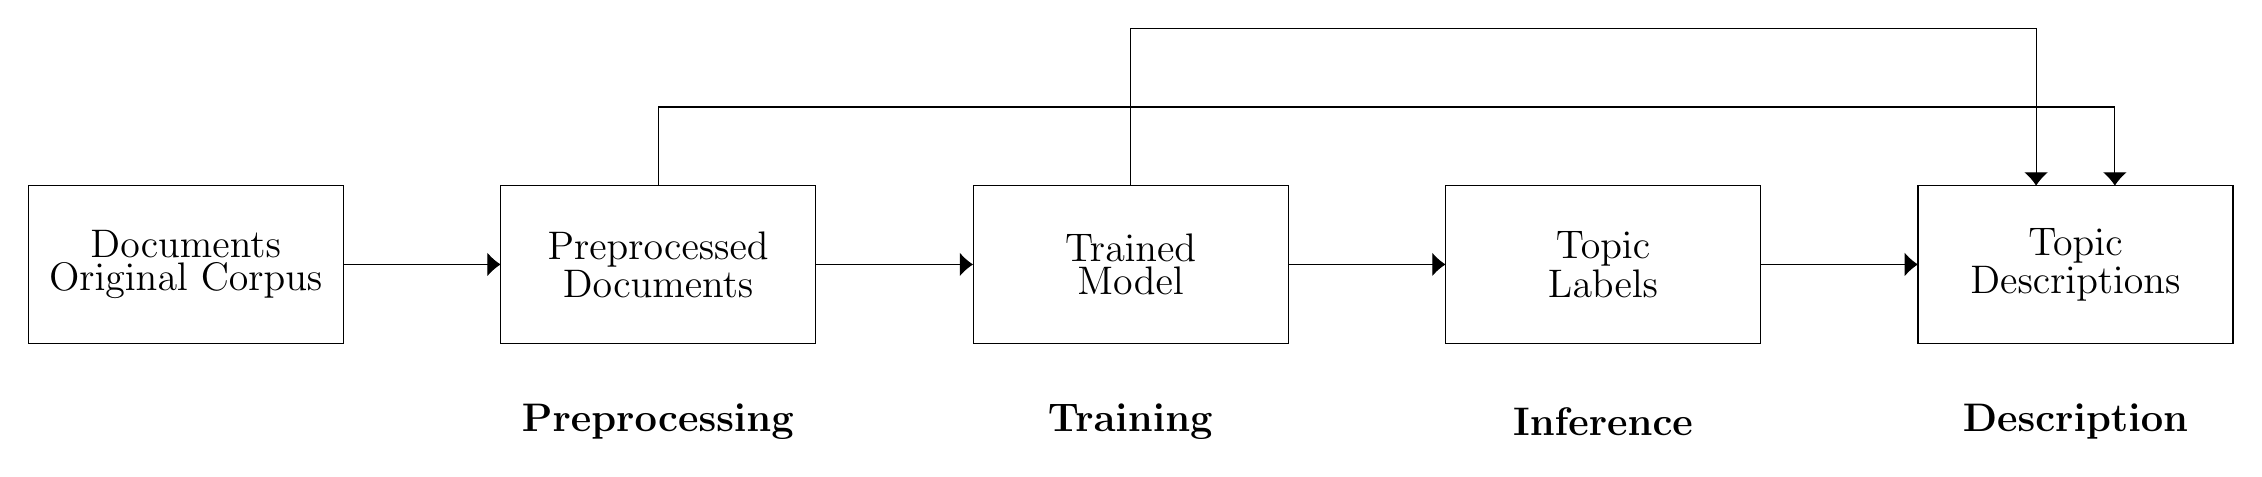
\begin{tikzpicture}[grow=right]

    \draw (0, 0) rectangle (4,2) node[pos=0.5, align=center]{\Large Documents\\\Large Original Corpus};
    \draw (6, 0) rectangle (10,2) node[pos=0.5, align=center]{\Large Preprocessed\\\Large Documents};
    \draw (12, 0) rectangle (16,2) node[pos=0.5, align=center]{\Large Trained\\\Large Model};
    \draw (18, 0) rectangle (22,2) node[pos=0.5, align=center]{\Large Topic\\\Large Labels};
    \draw (24, 0) rectangle (28,2) node[pos=0.5, align=center]{\Large Topic\\\Large Descriptions};

    \node[align=center] at (8, -1) {\Large\textbf{Preprocessing}};
    \node[align=center] at (14, -1) {\Large\textbf{Training}};
    \node[align=center] at (20, -1) {\Large\textbf{Inference}};
    \node[align=center] at (26, -1) {\Large\textbf{Description}};

    \draw[-{Latex[width=3mm]}] (4, 1) -- (6, 1);
    \draw[-{Latex[width=3mm]}] (10, 1) -- (12, 1);
    \draw[-{Latex[width=3mm]}] (16, 1) -- (18, 1);
    \draw[-{Latex[width=3mm]}] (22, 1) -- (24, 1);

    \draw[-{Latex[width=3mm]}] (8, 2) -- (8, 3) -- (26.5, 3) -- (26.5, 2);
    \draw[-{Latex[width=3mm]}] (14, 2) -- (14, 4) -- (25.5, 4) -- (25.5, 2);

\end{tikzpicture}
\end{document}